\documentclass[12pt]{ctexart}

\usepackage{graphicx}
\usepackage{amsthm}
\usepackage{amsmath}
\usepackage{amssymb}
\usepackage[hmargin=1.1in,vmargin=1in]{geometry}
\usepackage{indentfirst}
\usepackage[defaultmono,scale=0.85]{droidsansmono}
\usepackage{multirow}
\usepackage[outputdir={dotpics/}]{dot2texi}
\usepackage{tikz}
\usepackage{subfig}
\usepackage{booktabs}
\usepackage{xcolor}
\usepackage[luatex,colorlinks=true]{hyperref}

\fontsize{14pt}{1.0}
\usetikzlibrary{graphdrawing, graphs, quotes, automata, positioning}
\usegdlibrary{layered, trees}

\newlength{\blanklength}
\setlength{\blanklength}{40ex}

\providecommand{\thetitle}{第四章作业}
\providecommand{\theauthor}{Sparky\_14145}
\providecommand{\thestudentID}{71XXXXXX}
\providecommand{\theemail}{Sparky\_14145@outlook.com}
\providecommand{\theinstitution}{软件工程学院}

% \input{personal_info/info.tex}

\providecommand{\blankToFill}[1]{
    \parbox[t][3ex]{\blanklength}{
        \makebox[\blanklength]{#1}\\[0pt]
        \rule[2ex]{\blanklength}{0.1ex}
    }
}

\providecommand{\makecover}{\begin{titlepage}
    \noindent
    {课程作业} \\[2pt]
    {\large \bfseries 东南大学}

    \vspace*{70pt}
    \begin{center}
        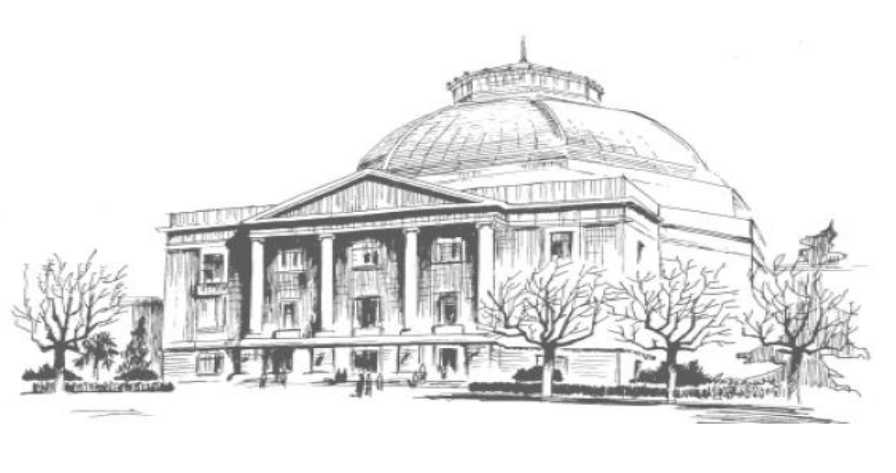
\includegraphics[width=0.9\textwidth]{pics/cover.png} \\[2pt]
        \textsc{\Huge Principles of Compilers}\\[10pt]
        \begin{tabular}[c]{rc}
            题目    & \blankToFill{\thetitle} \\
            日期    & \blankToFill{\today} \\
            姓名    & \blankToFill{\theauthor\footnotemark} \\
            学号    & \blankToFill{\thestudentID} \\
            院系    & \blankToFill{\theinstitution}
        \end{tabular}
        \rmfamily
    \end{center}
    \footnotetext{\theemail}
\end{titlepage}}

\newcommand{\red}[1]{{\color{red}#1}}

\begin{document}
    \makecover

    \tableofcontents

    \newpage
    \section{T 4.2.1}

    考虑上下文无关文法:

    \[S \to S\;S\;+|\;S\;S*|\;a\]

    以及串 $aa+a*$

    \begin{enumerate}
        \item 给出这个串的一个最左推导。
        \item 给出这个串的一个最右推导。
        \item 给出这个串的一棵语法分析树。
        \item 这个文法是否为二义性的?证明你的回答。
        \item 描述这个文法生成的语言。
    \end{enumerate}

    \emph{解:}
    \begin{enumerate}
        \item \begin{align*}
            S   &\underset{lm}\Rightarrow S\;S*     \\
                &\underset{lm}\Rightarrow S\;S+S*   \\
                &\underset{lm}\Rightarrow a\;S+S*   \\
                &\underset{lm}\Rightarrow a\;a+S*   \\
                &\underset{lm}\Rightarrow a\;a+a*
        \end{align*}
        \item \begin{align*}
            S   &\underset{rm}\Rightarrow S\;S*     \\
                &\underset{rm}\Rightarrow S\;a*     \\
                &\underset{rm}\Rightarrow S\;S+a*   \\
                &\underset{rm}\Rightarrow S\;a+a*   \\
                &\underset{rm}\Rightarrow a\;a+a*
        \end{align*}
        \item 见图 \ref{fig:t1-parse-tree}。
        \item 这个文法无二义性。
        \item 一个后缀表达式的集合,其中运算符为 $+$ 与 $*$,操作数为 $a$。
    \end{enumerate}

    \begin{figure}[hp]
        \centering
        \begin{tikzpicture}[tree layout,scale=1.5]
            \graph[math nodes]{
                S1[as=$S$] -- {
                    S2[as=$S$] -- {
                        S3[as=$S$] -- a1[as=$a$],
                        S4[as=$S$] -- a2[as=$a$],
                        +
                    },
                    S5[as=$S$] -- a3[as=$a$], 
                    *
                }
            };
        \end{tikzpicture}
        \caption{T4.2.1 的语法分析树}
        \label{fig:t1-parse-tree}
    \end{figure}

    \clearpage
    \newpage
    \section{T 4.2.3}

    为下面的语言设计文法:

    \begin{enumerate}
        \item[(a)] 所有由 0 和 1 组成且每个 0 之后至少跟着一个 1 的串的集合。
        \item[(b)] 所有由 0 和 1 组成的回文的集合。
        \item[(c)] 所有由 0 和 1 组成的且 0 和 1 的个数相同的集合。
        \item[(e)] 所有由 0 和 1 组成的且其中不包含子串 011 的串的集合。
    \end{enumerate}

    \emph{解:} 我们认为空串为由 0 个 0 和 0 个 1 组成的串。
    \begin{enumerate}
        \item[(a)] \begin{align*}
            S \to S\;1\;|\;S\;0\;1|\;\varepsilon
        \end{align*}
        \item[(b)] \[
            S \to 0\;S\;0\;|\;1\;S\;1\;|\;\varepsilon
        \]
        \item[(c)] \[
            S \to 0\;S\;1\;|\;1\;S\;0\;|\;S\;S\;|\;\varepsilon
        \]
        \item[(e)] \begin{align*}
            S   &\to S_1\;|\;S_2\;|\;S_3    \\
            S_1 &\to \varepsilon\;|\;S_1\;1 \\
            S_2 &\to S\;0                   \\
            S_3 &\to S_2\;1
        \end{align*}
    \end{enumerate}

    \clearpage
    \newpage
    \section{T 4.4.1}

    为下面每一个文法设计一个预测分析器,并给出预测分析表。你可能需要先对文法进行提取左公因子或消除左递归的操作。

    \begin{enumerate}
        \item[(a)] $S \to 0\;S\;1\;|\;0\;1$
        \item[(c)] $S \to S\;(\;S\;)\;S\;|\;\varepsilon$
        \item[(e)] \begin{align*}
            S &\to (\;L\;)\;|\;a \\
            L &\to L\;,\;S\;|\;S
        \end{align*}
    \end{enumerate}

    \emph{解:}
    \begin{enumerate}
        \item[(a)] 消除左递归并提取左公因子之后得到文法:
        \begin{align*}
            S   &\to 0\;S' \\
            S'  &\to 1\;|\;0\;S'\;1 
        \end{align*}
        再构造预测分析表,如表 \ref{tab:t3-1} 所示。
        \item[(c)] 消除左递归并提取左公因子之后得到文法:
        \begin{align*}
            S   &\to S'             \\
            S'  &\to (\;S\;)\;S\;S'\;|\;\varepsilon
        \end{align*}
        再构造预测分析表,如表 \ref{tab:t3-2} 所示。

        通过表 \ref{tab:t3-2} 可以发现,该文法有二义性。
        \item[(e)] 消除左递归并提取左公因子之后得到文法:
        \begin{align*}
            S   &\to (\;L\;)\;|\;a  \\
            L   &\to S\;L'          \\
            L'  &\to \;,\;S\;L'\;|\;\varepsilon
        \end{align*}
    \end{enumerate}

    \begin{table}[hp]
        \centering
        \caption{T4.4.1(a) 预测分析表}
        \label{tab:t3-1}
        \begin{tabular}{|*4{c|}}
            \hline
            \multirow{2}{*}{非终结符号} & \multicolumn{3}{c|}{输入符号} \\ \cline{2-4}
             & 0 & 1 & \$ \\ \hline
            $S$ & $S \to 0\;S'$ &  &  \\
            $S'$ & $S' \to 0\;S\;1$ & $S' \to 1$ &  \\ \hline
        \end{tabular}
    \end{table}

    \begin{table}[hp]
        \centering
        \caption{T4.4.1(c) 预测分析表}
        \label{tab:t3-2}
        \begin{tabular}{|*4{c|}}
            \hline
            \multirow{2}{*}{非终结符号} & \multicolumn{3}{c|}{输入符号} \\ \cline{2-4}
             & ( & ) & \$ \\ \hline
            $S$ & $S \to S'$ & $S \to S'$ & $S \to S'$ \\
            $S'$ & $S' \to (\;S\;)\;S\;S'\;|\;\varepsilon$ & $S' \to \varepsilon$ & $S' \to \varepsilon$ \\ \hline
        \end{tabular}
    \end{table}

    \begin{table}[hp]
        \centering
        \caption{T4.4.1(e) 预测分析表}
        \label{tab:t3-3}
        \begin{tabular}{|*{6}{c|}}
            \hline
            \multirow{2}{*}{非终结符号} & \multicolumn{5}{c|}{输入符号} \\ \cline{2-6}
             & $a$ & ( & ) & , & \$ \\ \hline
            $S$ & $S \to a$ & $S \to (\;L\;)$ & & &  \\
            $L$ & $L \to S\;L'$ & $L\to S\;L'$ & & & \\
            $L'$ & $$ & $$ & $L' \to \varepsilon$ & $L' \to\;,\;S\;L'$ & \\ \hline
        \end{tabular}
    \end{table}

    \clearpage
    \newpage
    \section{T 4.6.5}

    说明下面文法

    \begin{equation}
        \label{eq:t4}
        \begin{aligned}
            S &\to A\;a\;A\;b\;|\;B\;b\;B\;a    \\
            A &\to \varepsilon                  \\
            B &\to \varepsilon
        \end{aligned}
    \end{equation}

    是 LL(1) 的,但不是 SLR(1) 的。

    \begin{proof}
        首先证明文法 \eqref{eq:t4} 是 LL(1) 的:
        \begin{enumerate}
            \item 与 $A$ 和 $B$ 相关的产生式各只有一个,且与 $S$ 相关的两个产生式分别只能推导出一个串 $ab$ 与 $ba$,两者没有公共前缀,故 LL(1) 的条件 (1) 满足;
            \item 与 $A$ 和 $B$ 相关的产生式各只有一个,且与 $S$ 相关的产生式显然不会推导出 $\varepsilon$,故 LL(1) 的条件 (2) 满足;
            \item 与 $A$ 和 $B$ 相关的产生式各只有一个,且与 $S$ 相关的两个产生式均无法推导出 $\varepsilon$,故 LL(1) 的条件 (3) 满足。
        \end{enumerate}
        综上所述,文法 \eqref{eq:t4} 是 LL(1) 的。

        再证明文法 \eqref{eq:t4} 不是 SLR(1) 的:\\
        首先构造增广文法 $G'$,如文法 \eqref{eq:t4-1} 所示:
        \begin{equation}
            \label{eq:t4-1}
            \begin{aligned}
                S'  &\to S          &(1)    \\
                S   &\to A\;a\;A\;b &(2)    \\
                S   &\to B\;b\;B\;a &(3)    \\
                A &\to \varepsilon  &(4)    \\
                B &\to \varepsilon  &(5)
            \end{aligned}
        \end{equation}
        然后得到文法 $G'$ 的各个项集,如表 \ref{tab:t4-coll} 所示。\\
        并构造出如表 \ref{tab:t4-slr} 所示的语法分析表。\\
        观察表 \ref{tab:t4-slr} 可知,ACTION[0, $a$] 与 ACTION[0, $b$] 存在冲突,因此文法 \eqref{eq:t4} 不是 SLR(1) 的。

        故文法 \eqref{eq:t4} 是 LL(1) 的,但不是 SLR(1) 的。
    \end{proof}

    \begin{table}[hp]
        \centering
        \caption{T4.6.5 的 LR(1) 项集族}
        \label{tab:t4-coll}
            \begin{tabular}{|c|c|}
                \hline
                项名称 & 项内容 \\ \hline
                \multirow{5}{*}{$I_0$} & $S' \to \cdot S$ \\
                 & $S \to \cdot A\;a\;A\;b$ \\
                 & $S \to \cdot B\;b\;B\;a$ \\
                 & $A \to \cdot$ \\
                 & $B \to \cdot$ \\ \hline
                \multirow{1}{*}{$I_1$} & $S' \to S \cdot$ \\ \hline
                \multirow{1}{*}{$I_2$} & $S \to A \cdot a\;A\;b$ \\ \hline
                \multirow{1}{*}{$I_3$} & $S \to B \cdot b\;B\;a$ \\ \hline
                \multirow{2}{*}{$I_4$} & $S \to A\;a \cdot A\;b$ \\
                 & $A \to \cdot$ \\ \hline
                \multirow{2}{*}{$I_5$} & $S \to B\;b \cdot B\;a$ \\
                 & $B \to \cdot$ \\ \hline
                \multirow{1}{*}{$I_6$} & $S \to A\;a\;A \cdot b$ \\ \hline
                \multirow{1}{*}{$I_7$} & $S \to B\;b\;B \cdot a$ \\ \hline
                \multirow{1}{*}{$I_8$} & $S \to A\;a\;A\;b \cdot $ \\ \hline
                \multirow{1}{*}{$I_9$} & $S \to B\;b\;B\;a \cdot $ \\ \hline
            \end{tabular}
    \end{table}

    \begin{table}[hp]
        \centering
        \caption{T4.6.5 的 SLR 语法分析表}
        \label{tab:t4-slr}
        \begin{tabular}{|*{1}{c}|*{3}{c}|*{4}{c}|}
            \hline
            \multirow{2}{*}{状态} & \multicolumn{3}{c|}{ACTION} & \multicolumn{4}{c|}{GOTO} \\ \cline{2-8}
             & $a$ & $b$ & \$ & $S'$ & $S$ & $A$ & $B$ \\ \hline
            0 & r4, r5 & r4, r5 & & & 1 & 2 & 3 \\
            1 & & & acc & & & & \\
            2 & s4 & & & & & & \\
            3 & & s5 & & & & & \\
            4 & r4 & r4 & & & & 6 & \\
            5 & r5 & r5 & & & & & 7 \\
            6 & s8 & & & & & & \\
            7 & & s9 & & & & & \\
            8 & & & r2 & & & & \\
            9 & & & r3 & & & & \\ \hline
        \end{tabular}
    \end{table}

    \clearpage
    \newpage
    \section{T 4.6.6}

    说明下面文法:

    \begin{equation}
        \label{eq:t5}
        \begin{aligned}
            S &\to S\;A\;|\;A \\
            A &\to a
        \end{aligned}
    \end{equation}

    是 SLR(1) 的,但不是 LL(1) 的。

    \begin{proof}
        从产生式 $S \to S\;A$ 可以看出,文法 \eqref{eq:t5} 存在左递归,故该文法不是 LL(1) 的。

        要证明文法 \eqref{eq:t5} 是 SLR(1) 的,先将文法改写为增广文法 $G'$:
        \begin{align*}
            S'  &\to S      &(1) \\
            S   &\to S\;A   &(2) \\
            S   &\to A      &(3) \\
            A   &\to a      &(4)
        \end{align*}
        然后构造其规范 LR(0) 项集族,如表 \ref{tab:t5-items} 所示。\\
        最后构造出如表 \ref{tab:t4-slr} 所示的语法分析表。观察可知表中不存在冲突,故文法 \eqref{eq:t5} 是 SLR(1) 的。

        综上所述,文法 \eqref{eq:t5} 是 SLR(1) 的,但不是 LL(1) 的。
    \end{proof}

    \begin{table}[hp]
        \centering
        \caption{T4.6.6 的 LR(0) 项集族}
        \label{tab:t5-items}
        \begin{tabular}{|c|c|}
            \hline
            项名称 & 项内容 \\ \hline
            \multirow{4}{*}{$I_0$} & $S' \to \cdot S$ \\
             & $S \to \cdot S\;A$ \\
             & $S \to \cdot A$ \\
             & $A \to \cdot a$ \\ \hline
            \multirow{3}{*}{$I_1$} & $S' \to S \cdot$ \\
             & $S \to S \cdot A$ \\ 
             & $A \to \cdot a$ \\ \hline
            \multirow{1}{*}{$I_2$} & $S \to A \cdot$ \\ \hline
            \multirow{1}{*}{$I_3$} & $A \to a \cdot$ \\ \hline
            \multirow{1}{*}{$I_4$} & $S \to S\;A\cdot$ \\ \hline
        \end{tabular}
    \end{table}

    \begin{table}[hp]
        \centering
        \caption{T4.6.6 的 SLR 语法分析表}
        \label{tab:t5-slr}
        \begin{tabular}{|c|*{2}{c}|*{3}{c}|}
            \hline
            \multirow{2}{*}{状态} & \multicolumn{2}{c|}{ACTION} & \multicolumn{3}{c|}{GOTO} \\ \cline{2-6}
             & $a$ & \$ & $S'$ & $S$ & $A$ \\ \hline
            0 & s3 & & & 1 & 2 \\
            1 & & acc & & & 4 \\
            2 & r3 & r3 & & & \\
            3 & r4 & r4 & & & \\
            4 & r2 & r2 & & & \\ \hline
        \end{tabular}
    \end{table}

    \clearpage
    \newpage
    \section{构造 LR(1) 语法分析表}

    为下列语法创建 LR(1) 语法分析表:

    \begin{enumerate}
        \item $S \to 0\;S\;1\;|\;0\;1$
        \item $S \to S\;(\;S\;)\;S\;|\;\varepsilon$
        \item \begin{align*}
            S &\to \;(\;L\;)\;|\;a \\
            L &\to L\;,\;S\;|\;S
        \end{align*}
    \end{enumerate}

    \emph{解:}
    \begin{enumerate}
        \item 将文法改写为增广文法:
        \begin{align*}
            S' &\to S &(1) \\
            S &\to 0\;S\;1 &(2) \\
            S &\to 0\;1 &(3)
        \end{align*}
        然后得到如表 \ref{tab:t6-1-items} 所示的 LR(1) 项集族,并构造出如表 \ref{tab:t6-1-lr1} 所示的 LR(1) 语法分析表。
        \item 将文法改写为增广文法:
        \begin{align*}
            S' &\to S &(1) \\
            S &\to S\;(\;S\;)\;S &(2) \\
            S &\to \varepsilon &(3)
        \end{align*}
        然后得到如表 \ref{tab:t6-2-items} 所示的 LR(1) 项集族,并构造出如表 \ref{tab:t6-2-lr1} 所示的 LR(1) 语法分析表。
        (我知道这两个表是错的,懒得管了,太累了)
        \item 将文法改写为增广文法:
        \begin{align*}
            S' &\to S &(1) \\
            S  &\to (\;L\;) &(2) \\
            S  &\to a &(3) \\
            L  &\to L\;,\;S &(4) \\
            L  &\to S &(5)
        \end{align*}
        然后得到如表 \ref{tab:t6-3-items} 所示的 LR(1) 项集族,并构造出如表 \ref{tab:t6-3-lr1} 所示的 LR(1) 语法分析表。(注意:为了和文法中原有的`,'区分,这里使用符号`;'来分隔项与向前看符号)
    \end{enumerate}

    \begin{table}[hp]
        \centering
        \caption{T6(1) 的 LR(1) 项集族}
        \label{tab:t6-1-items}
        \begin{tabular}{|c|c|}
            \hline
            项集名称 & 项集内容 \\ \hline
            \multirow{3}{*}{$I_0$} & $[S' \to \cdot S, \$]$ \\
             & $[S \to \cdot 0\;S\;1, \$]$ \\
             & $[S \to \cdot 0\;1, \$]$ \\ \hline
            \multirow{1}{*}{$I_1$} & $[S' \to S \cdot, \$]$ \\ \hline
            \multirow{4}{*}{$I_2$} & $[S \to 0 \cdot S\;1, \$]$ \\
             & $[S \to 0 \cdot 1, \$]$ \\
             & $[S \to \cdot 0\;S\;1, 1]$ \\
             & $[S \to \cdot 0\;1, 1]$ \\ \hline
            \multirow{1}{*}{$I_3$} & $[S \to 0\;S \cdot 1, \$]$ \\ \hline
            \multirow{1}{*}{$I_4$} & $[S \to 0\;S\;1\cdot, \$]$ \\ \hline
            \multirow{1}{*}{$I_5$} & $[S \to 0\;1\cdot, \$]$ \\ \hline
            \multirow{4}{*}{$I_6$} & $[S \to 0 \cdot S\;1, 1]$ \\
             & $[S \to 0 \cdot 1, 1]$ \\
             & $[S \to \cdot 0\;S\;1, 1]$ \\
             & $[S \to \cdot 0\;1, 1]$ \\ \hline
            \multirow{1}{*}{$I_7$} & $[S \to 0\;1\cdot, 1]$ \\ \hline
            \multirow{1}{*}{$I_8$} & $[S \to 0\;S \cdot 1, 1]$ \\ \hline
            \multirow{1}{*}{$I_9$} & $[S \to 0\;S\;1\cdot, 1]$ \\ \hline
        \end{tabular}
    \end{table}

    \begin{table}
        \centering
        \caption{T6(1) 的 LR(1) 语法分析表}
        \label{tab:t6-1-lr1}
        \begin{tabular}{|c|*{3}{c}|*{2}{c}|}
            \hline
            \multirow{2}{*}{状态} & \multicolumn{3}{c|}{ACTION} & \multicolumn{2}{c|}{GOTO} \\ \cline{2-6}
             & 0 & 1 & \$ & $S'$ & $S$ \\ \hline
            0 & s2 & & & & 1 \\
            1 & & & acc & & \\
            2 & s5 & s6 & & & 3 \\
            3 & & s4 & & & \\
            4 & & & r2 & & \\
            5 & & & r3 & & \\
            6 & s6 & s7 & & & 8 \\
            7 & & r3 & & & \\
            8 & & s9 & & & \\
            9 & & r2 & & & \\ \hline
        \end{tabular}
    \end{table}

    \begin{table}[hp]
        \centering
        \caption{T6(2) 的 LR(1) 项集族}
        \label{tab:t6-2-items}
        \begin{tabular}{|c|cc|}
            \hline
            项集名称 & \multicolumn{2}{c|}{项集内容} \\ \hline
            \multirow{3}{*}{$I_0$} & $[S' \to \cdot S, \$]$ & $[S \to \cdot S\;(\;S\;)\;S, \$]$ \\
             & $[S \to \cdot, \$]$ & $[S \to \cdot S\;(\;S\;)\;S, (]$ \\
             & $[S \to \cdot, (]$ & \\ \hline
            \multirow{2}{*}{$I_1$} & $[S' \to S \cdot, \$]$ & $[S \to S \cdot (\;S\;)\;S, \$]$ \\
             & $[S \to S \cdot (\;S\;)\;S, (]$ & \\\hline
            \multirow{2}{*}{$I_2$} & $[S \to S\;(\cdot S\;)\;S, \$]$ & $[S \to S\;(\cdot S\;)\;S, (]$ \\ 
             & $[S \to \cdot S\;(\;S\;)\;S, )]$ & $[S \to \cdot, )]$ \\ \hline
            \multirow{2}{*}{$I_3$} & $[S \to S\;(\;S\cdot)\;S, \$]$ & $[S \to S\;(\;S\cdot)\;S, (]$ \\ 
             & $[S \to S \cdot (\;S\;)\;S, )]$ & \\\hline
            \multirow{3}{*}{$I_4$} & $[S \to S\;(\;S\;)\cdot S, \$]$ & $[S \to S\;(\;S\;)\cdot S, (]$ \\ 
             & $[S \to \cdot S\;(\;S\;)\;S, \$]$ & $[S \to \cdot, \$]$ \\
             & $[S \to \cdot S\;(\;S\;)\;S, (]$ & $[S \to \cdot, (]$ \\ \hline
            \multirow{2}{*}{$I_5$} & $[S \to S\;(\;S\;)\;S\cdot, \$]$ & $[S \to S\;(\;S\;)\;S\cdot, (]$ \\
             & $[S \to S \cdot (\;S\;)\;S, \$]$ & $[S \to S \cdot (\;S\;)\;S, (]$ \\ \hline
            \multirow{1}{*}{$I_6$} & $[S \to S\;(\cdot S\;)\;S, )]$ & $[S \to \cdot, )]$ \\ \hline
            \multirow{1}{*}{$I_7$} & $[S \to S\;(\;S \cdot)\;S, )]$ & $[S \to \cdot S\;(\;S\;)\;S, )]$ \\ \hline
            \multirow{3}{*}{$I_8$} & $[S \to S\;(\;S\;)\cdot S, )]$ & $[S \to \cdot S\;(\;S\;)\;S, )]$ \\
             & $[S \to \cdot, )]$ & $[S \to \cdot S\;(\;S\;)\;S, (]$ \\
             & $[S \to \cdot, (]$ & \\ \hline
            \multirow{2}{*}{$I_9$} & $[S \to S\;(\;S\;)\;S\cdot, )]$ & $[S \to S \cdot (\;S\;)\;S, )]$ \\
             & $[S \to S \cdot (\;S\;)\;S, (]$ & \\ \hline
        \end{tabular}
    \end{table}

    \begin{table}
        \centering
        \caption{T6(2) 的 LR(1) 语法分析表}
        \label{tab:t6-2-lr1}
        \begin{tabular}{|c|*{3}{c}|*{2}{c}|}
            \hline
            \multirow{2}{*}{状态} & \multicolumn{3}{c|}{ACTION} & \multicolumn{2}{c|}{GOTO} \\ \cline{2-6}
             & ( & ) & \$ & $S'$ & $S$ \\ \hline
            0 & r3 & & r3 & & 1 \\
            1 & & & acc & & \\
            2 & s5 & s6 & & & 3 \\
            3 & & s4 & & & \\
            4 & & & r2 & & \\
            5 & & & r3 & & \\ \hline
        \end{tabular}
    \end{table}

    \begin{table}
        \centering
        \caption{T6(3) 的 LR(1) 项集族}
        \label{tab:t6-3-items}
        \begin{tabular}{|c|cc|}
            \hline
            项集名称 & \multicolumn{2}{c|}{项集内容} \\ \hline
            \multirow{2}{*}{$I_0$} & $[S' \to \cdot S; \$]$ & $[S \to \cdot (\;L\;); \$]$ \\
             & $[S \to \cdot a; \$]$ & \\ \hline
            \multirow{1}{*}{$I_1$} & $[S' \to S \cdot; \$]$ & \\ \hline
            \multirow{1}{*}{$I_2$} & $[S \to a\cdot; \$]$ & \\ \hline
            \multirow{3}{*}{$I_3$} & $[S \to (\cdot L\;); \$]$ & $[L \to \cdot L\;,\;S; )]$ \\
             & $[L \to \cdot S; )]$ & $[L \to \cdot L\;,\;S;\;,]$ \\
             & $[S \to \cdot (\;L\;); )]$ & $[S \to \cdot a; )]$ \\ \hline
            \multirow{2}{*}{$I_4$(I3-L)} & $[S \to (\;L \cdot ); \$]$ & $[L \to L \cdot,\;S; )]$ \\
             & $[L \to L \cdot,\;S;\;,]$ & \\ \hline
            \multirow{1}{*}{$I_5$(I4-))} & $[S \to (\;L\;)\cdot; \$]$ & \\ \hline
            \multirow{3}{*}{$I_6$(I4-,)} & $[L \to L\;,\cdot S;\;,]$ & $[S \to \cdot (\;L\;);\;,]$ \\
             & $[S \to \cdot a;\;,]$ & $[L \to L\;,\cdot S; )]$ \\
             & $[S \to \cdot (\;L\;); )]$ & $[S \to \cdot a; )]$ \\ \hline
            \multirow{1}{*}{$I_7$(I6-S)} & $[L \to L\;,\;S\cdot;\;,]$ & $[L \to L\;,\;S\cdot;\;)]$ \\ \hline
            \multirow{5}{*}{$I_8$(I6-()} & $[S \to (\cdot L\;);\;,]$ & $[L \to \cdot L\;,\;S; )]$ \\
             & $[L \to \cdot S; ,]$ & $[L \to \cdot L\;,\;S;\;,]$ \\
             & $[S \to \cdot (\;L\;); )]$ & $[S \to \cdot a; )]$ \\
             & $[S \to (\cdot L\;);\;)]$ & $[L \to \cdot S; )]$ \\
             & $[S \to \cdot a; ,]$ & $[S \to \cdot (\;L\;); ,]$ \\ \hline
            \multirow{2}{*}{$I_9$(I8-L)} & $[S \to (\;L \cdot ); ,]$ & $[L \to L \cdot,\;S; )]$ \\
            & $[L \to L \cdot,\;S;\;,]$ & $[S \to (\;L \cdot ); )]$ \\ \hline
            \multirow{1}{*}{$I_{10}$(I9-))} & $[S \to (\;L\;)\cdot; ,]$ & $[S \to (\;L\;)\cdot; )]$ \\ \hline
            \multirow{1}{*}{$I_{11}$(I8-a)} & $[S \to a\cdot; )]$ & $[S \to a\cdot;\;,]$ \\ \hline
            \multirow{1}{*}{$I_{12}$(I8-S)} & $[L \to S\cdot;)]$ & $[L \to S\cdot;\;,]$ \\ \hline
            \multirow{1}{*}{$I_{13}$(I3-S)} & $[L \to S\cdot;)]$ & \\ \hline
            \multirow{1}{*}{$I_{14}$(I3-a)} & $[S \to a\cdot;)]$ & \\ \hline
            \multirow{5}{*}{$I_{15}$(I3-()} & $[S \to (\cdot L\;);)]$ & $[L \to \cdot S;)]$ \\
             & $[L \to \cdot L\;,\;S;)]$ & $[S \to \cdot a; )]$ \\
             & $[S \to \cdot (\;L\;); )]$ & $[L \to \cdot L\;,\;S; ,]$ \\
             & $[L \to \cdot S; ,]$ & $[S \to \cdot (\;L\;); ,]$ \\
             & $[S \to \cdot a; ,]$ & \\ \hline
            \multirow{2}{*}{$I_{16}$(I15-L)} & $[L \to L \cdot,\;S; )]$ & $[L \to L \cdot,\;S;\;,]$ \\
             & $[S \to (\;L \cdot ); )]$ & \\ \hline
            \multirow{1}{*}{$I_{17}$(I16-))} & $[S \to (\;L\;)\cdot; )]$ & \\ \hline
        \end{tabular}
    \end{table}

    \begin{table}
        \centering
        \caption{T6(3) 的 LR(1) 语法分析表}
        \label{tab:t6-3-lr1}
        \begin{tabular}{|c|*{5}{c}|*{3}{c}|}
            \hline
            \multirow{2}{*}{名称} & \multicolumn{5}{c|}{ACTION} & \multicolumn{3}{c|}{GOTO} \\ \cline{2-9}
             & $a$ & ( & ) & , & \$ & $S'$ & $S$ & $L$ \\ \hline
            0 & s2 & s3 & & & & & 1 & \\
            1 & & & & & acc & & & \\
            2 & & & & & r3 & & & \\
            3 & s14 & s15 & & & & & 13 & 4 \\
            4 & & & s5 & s6 & & & & \\
            5 & & & & & r2 & & & \\
            6 & s11 & s8 & & & & & 7 & \\
            7 & & & r4 & r4 & & & & \\
            8 & s11 & s8 & & & & & 12 & 9 \\
            9 & & & s10 & s6 & & & & \\
            10 & & & r2 & r2 & & & & \\
            11 & & & r3 & r3 & & & & \\
            12 & & & r5 & r5 & & & & \\
            13 & & & r5 & & & & & \\
            14 & & & r3 & & & & & \\
            15 & s11 & s8 & & & & & 12 & 16 \\
            16 & & & s17 & s6 & & & & \\
            17 & & & r2 & & & & & \\ \hline
        \end{tabular}
    \end{table}
\end{document}
